\chapter{Arhitectura soluţiei}

\section{Prezentare generală}

In vederea implementării sistemului s-au identificat următoarele elemente componente esenţiale: 
\begin{itemize}
\item \textbf{Canalul de date:} reprezinta elementul de baza a sistemului, care asigura recepţia, persistenta si emiterea de date. Datele dintr-un canal trebuie sa respecte un format prestabilit la crearea canalului. Pentru transformarea datelor in formatul stabilit, se poate introduce un bloc de pre-procesarea care transforma datele din un format brut in formatul standard.
\item \textbf{Blocul de intrare date:} elementul de intrare, alcătuit din mai multe canale de date. Blocurile de intrare permit gruparea mai multor canale de date într-o structura unica.   
\item \textbf{Blocul de procesare:} elementul dinamic al aplicaţiei, ce aplica transformări asupra datelor. Un bloc de procesare primeşte ca intrări mai multe canale de date, si are la ieşire un alt canal de date. Utilizatorul poate folosi blocuri standard, existente in sistem, sau poate implementa blocuri noi direct in interfaţa programului.
\item \textbf{Diagrama funcţie bloc(FBD):}  foloseşte blocuri de intrare, canale de date si blocuri de procesare pentru a descrie o funcţie complexa intre intrări si o ieşire. Aceste diagrame folosesc la date aflate pe canale de date, care sunt trimise către blocuri de procesare si, la final se obţine un singur rezultat care este salvat pe un canal de date.
\end{itemize}

\section{Punctul de date}

Punctul de date reprezinta elementul constructiv al sistemul, care este obiectul procesării, stocării si distribuţiei este punctul de date. 
Sistemul accepta intern date in formatele: 
\begin{wrapfigure}{r}{0.38\textwidth}
	\centering
	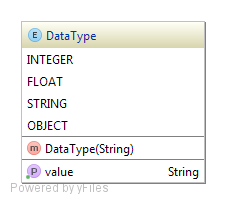
\includegraphics[width=0.38\textwidth]{dataType}
	\caption{Tipurile de date acceptate in sistem}
\end{wrapfigure}
\begin{itemize}
	\item \textbf{Întreg}: numere de la $-2^{63}$ la $2^{63} -1$, fără virgula, foloseşte \textit{Long} pentru reprezentare interna;
	\item \textbf{Real}: numere cu virgula, având dubla precizie, reprezentate cu 64-bit conform standardului \autocite{4610935} IEEE 754  foloseşte \textit{Double} pentru reprezentare interna;
	\item \textbf{Sir de caractere}: Un sir de fără limite a lungimii, care trebuie formatat conform \autocite{rfc4627}. 
	\item \textbf{Obiect}: Un obiect Java serializat in text. Intern, asemănător cu tipul de date String. 
\end{itemize}

\begin{figure}[h]
	\centering
	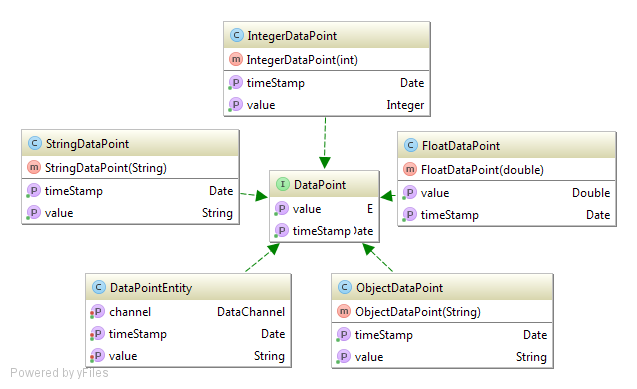
\includegraphics[width=0.93\textwidth]{dataPoint}
	\caption{Clasele care implementează interfaţa DataPoint}
\end{figure}

\section{Canalul de date}

Canalul de date este entitatea care asigura primirea, stocarea si distribuţia datelor. Cele trei funcţii sunt realizate complet separat, comunicarea intre modulele care implementează aceste funcţii fiind făcută pe baza de evenimente.
\begin{figure}[h]
	\centering
	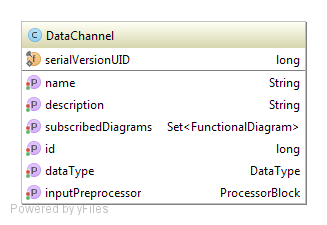
\includegraphics[width=0.6\textwidth]{dataChannel}
	\caption{Clasa DataChannel}
\end{figure}
\subsection{Primirea datelor}
Primirea datelor se face prin intermediul unei interfeţe de transfer a stării (REST). Mai multe formate sunt incluse pentru integrarea mai uşoară cu sisteme deja existente. Astfel, au fost implementate mai multe procesoare care primesc date atât într-un format special, cat si in formate standard in industrie.
Astfel, doua modalităţi de trimitere a datelor exista in sistem.
\begin{itemize}
	\item Trimitere către un singur canal, un singur punct odată: pe baza serviciului\\ \textit{/api/put/{inputId}/{channelId}/{data}}. Acest serviciu adaugă un singur punct in baza de date, la momentul curent. Folosit pentru sisteme care trimit date rar, si nu trebuie sa se tina cont de data locala de pe device-ul care a trimis punctul de date.
	\item In formatul standard folosit de openTDSB in care au fost introduse următoarele modificări care păstrează totuşi compatibilitatea: metricile reprezinta numele canalului, iar tag-urile sunt opţionale. Se acceptat atât formatul in care într-o cerere se afla un singur punct, cat si formatul cu o lista de puncte. Canalele dintr-o cere multidimensionala nu trebuie sa facă parte din acelaşi bloc de intrare. Acest mod de introducere a datelor este sugerat pentru sistemele care folosesc mai multe canale de date si care trimit seturi de date mai mari printr-o singura cerere. Spre exemplu, un dispozitiv poate trimite date de pe mai multi senzori, si poate stoca local mai multe măsurători pe acelaşi senzor pentru a trimite toate datele odată.
\end{itemize}
